\section{Experiments}
\label{s:expt}




\begin{table}[tb]
\begin{center}
\footnotesize
\caption{Lineage Strategies for experiments.}
  \begin{tabular}{ | l | l | }
    \hline
    {\bf Strategy} &  {\bf Description} \\ \hline \hline
    \multicolumn{2}{|c|}{\bf Astronomy Benchmark} \\ \hline
    BlackBox & All operators store black-box lineage \\ \hline
    BlackBoxOpt & Like BlackBox, uses mapping lineage for built-in-operators.\\ \hline
    FullOne & Like BlackBoxOpt, but uses FullOne for UDFs.\\ \hline
    FullMany & Like FullOne, but uses FullMany for UDFs.\\ \hline
    Subzero & Like FullOne, but stores composite lineage\\
            & using PayOne for UDFs.\\ \hline
    \multicolumn{2}{|c|}{\bf Genomics Benchmark} \\ \hline
    BlackBox & UDFs store black-box lineage \\ \hline
    FullOne & UDFs store backward optimized FullOne\\ \hline
    FullMany & UDFs store backward optimized FullMany\\ \hline
    FullForw & UDFs store forward optimized FullOne\\ \hline
    FullBoth & UDFs store FullForw and FullOne \\ \hline
    PayOne & UDFs store PayOne\\ \hline
    PayMany & UDFs store PayMany\\ \hline
    PayBoth & UDFs store PayOne and FullForw\\ \hline
\end{tabular}
\end{center}
\label{t:strats}
\end{table}

In the following subsections, we first describe how \sys{} optimizes the
storage strategies for the real-world benchmarks described in
Section~\ref{s:usecases}, then compare several of  our lineage storage
techniques with black-box level only techniques.  The astronomy benchmark shows
how our region lineage techniques improve over cell-level and black-box
strategies on  an image processing workflow.   The genomics benchmark
illustrates the complexity in determining an optimal lineage strategy and that
the the optimizer is able to  choose an effective strategy within user
constraints.


Overall, our findings are that:
\begin{itemize}

\item An optimal strategy heavily relies on operator properties such as fanin,
    and fanout, the specific lineage queries, and query execution-time
    optimizations.  The difference between a sub-optimal and optimal strategy
    can be so large that an optimizer-based approach is crucial.

\item Payload, composite, and mapping lineage are extremely effective and
    low overhead techniques that greatly improve query performance, and are
    applicable across a number of scientific domains.

\item  \sys{} can improve the LSST benchmark queries by up to 10$\times$
    compared to naively storing the region lineage (similar to what
    cell-level approaches would do) and up to 255$\times$ faster than black-box
    lineage.   The runtime and storage overhead of the optimal scheme is up to
    30 and 70$\times$ lower than cell-level lineage, respectively, and only
    1.49 and 1.95$\times$ higher than executing the workflow.

\item Even though the genomics benchmark executes operators very quickly,
    \sys{} can find the optimal mix of black-box and region lineage that scales
    to the amount of available storage.  \sys{} uses a black-box only strategy
    when the available storage is small, and switches from space-efficient to
    query-optimized encodings with looser constraints.  When the storage
    constraints are unbounded, \sys{} improves forward queries by over
    500$\times$ and backward queries by 2-3$\times$.

\end{itemize}

The current prototype is written in Python and uses BerkeleyDB for the
persistent store, and libspatialindex for the spatial index.  The
microbenchmarks are run on a 2.3 GHz linux server with 24 GB of RAM, running
Ubuntu 2.6.38-13-server.  The benchmarks are run on a 2.3 GHz MacBook Pro with
8 GB of RAM, a 5400 RPM hard disk, running OS X 10.7.2.

\subsection{Astronomy Benchmark}





\begin{figure}[htb]
\advance\leftskip-.1in
\subfigure[Disk and runtime overhead]
{
    \label{f:overhead1}
     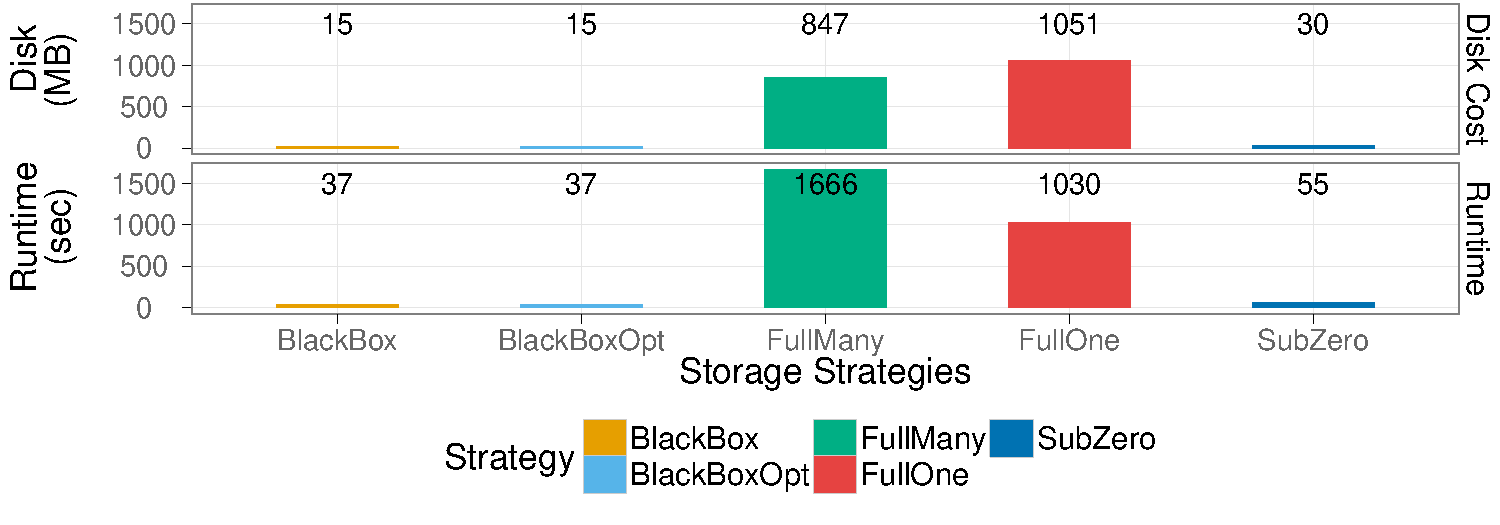
\includegraphics[width=3.5in,natwidth=10in,natheight=3.5in]{figures/lsst/overhead.pdf}
}
\subfigure[Query costs. Y-axes are log scale]
{
    \label{f:cost1}
    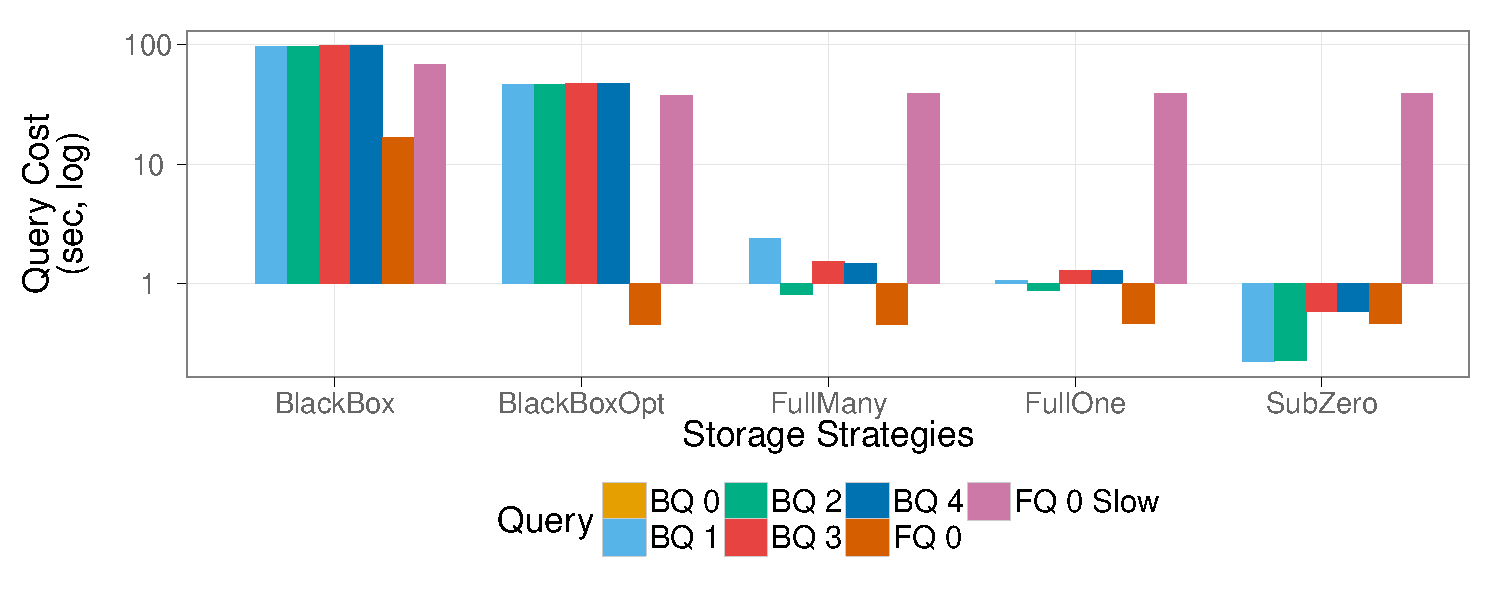
\includegraphics[width=3.5in,natwidth=10in,natheight=4in]{figures/lsst/cost.pdf}
}
\advance\rightskip-.2in
\caption{Astronomy Benchmark}
\label{f:lsst}
\end{figure}


In this experiment, we run the Astronomy workflow with  five backward
queries and one forward query as described in Section \ref{s:ucastro}.  The 22
built-in operators are all expressed as mapping operators and the UDFs consist
of one payload operator that detects celestial bodies and three composite
operators that detect and remove cosmic rays.  This workflow exhibits
considerable locality (stars only depend on neighboring pixels), sparsity
(stars are rare and small), and the queries are primarily backward queries.
Each workflow execution consumes two 512$\times$2000 pixel (8MB) images
(provided by LSST) as input, and we compare the strategies in Table \ref{t:strats}.

Figure \ref{f:overhead1} plots the disk and runtime overhead for each of the
strategies. $BlackBox$ and $BlackBoxOpt$ show the base cost to execute the
workflow and the size of the input arrays -- the goal is to be as close to
these bars as possible.  $FullOne$ and $FullMany$ both require considerable
storage space (66$\times$, 53$\times$) because the three cosmic ray operators
generate a region pair for every input and output pixel at the same
coordinates.  Similarly, both approaches incur 6$\times$ and 44$\times$ runtime
overhead to serialize and store them.  $FullMany$ must also
construct the spatial index on the output cells.  The \sys{} optimizer instead
picks composite lineage that only stores payload lineage for the small
number of cosmic rays and stars.  This reduces the runtime and disk overheads
to 1.49$\times$ and 1.95$\times$ the workflow inputs.  By comparison, this
storage overhead is negligible compared to the cost of storing the intermediate
and final results (which amount to 11.5$\times$ the input size).


Figure \ref{f:cost1} compares lineage query execution costs. $BQ~x$ and $FQ~x$
respectively stand for backward and forward query x.  All of the queries use
the entire array optimization described in Section \ref{s:qexec} whereas $FQ 0
Slow$ does not.  $BlackBox$ must re-run each operator and takes up to 100 secs
per query.  $BlackBoxOpt$ can avoid rerunning the mapping operators, but still
re-runs the computationally intensive UDFs.  Storing region lineage reduces
the cost of executing the backward queries by 34$\times$ ($FullMany$) and
$45\times$ ($FullOne$) on average.  \sys{} benefits from executing mapping
functions and reading a small amount of lineage data and executes 255$\times$
faster on average.  $FQ\ 0\ Slow$ illustrates how the all-to-all optimization
improves the query performance by 83$\times$ by avoiding fine-grained lineage
all-together.
















\subsection{Genomics Benchmark}




\begin{figure}[t]
\vspace{-.1in}
\advance\leftskip-.05in
\subfigure[Disk and runtime overhead]
{
    \label{f:goverhead}
    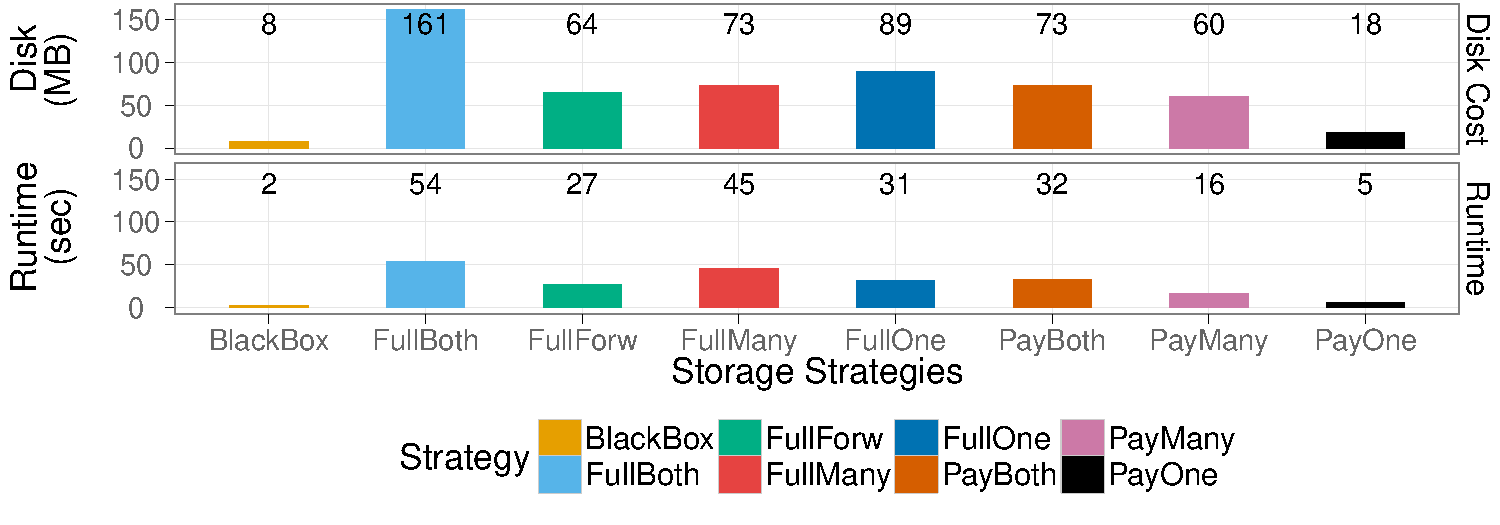
\includegraphics[width=3.5in,natwidth=10in,natheight=3.5in]{figures/genomics/overhead_noopt.pdf}
}
\subfigure[Query costs (static).  Y-axes are log scale.]
{
    \label{f:gcosts100_static}
     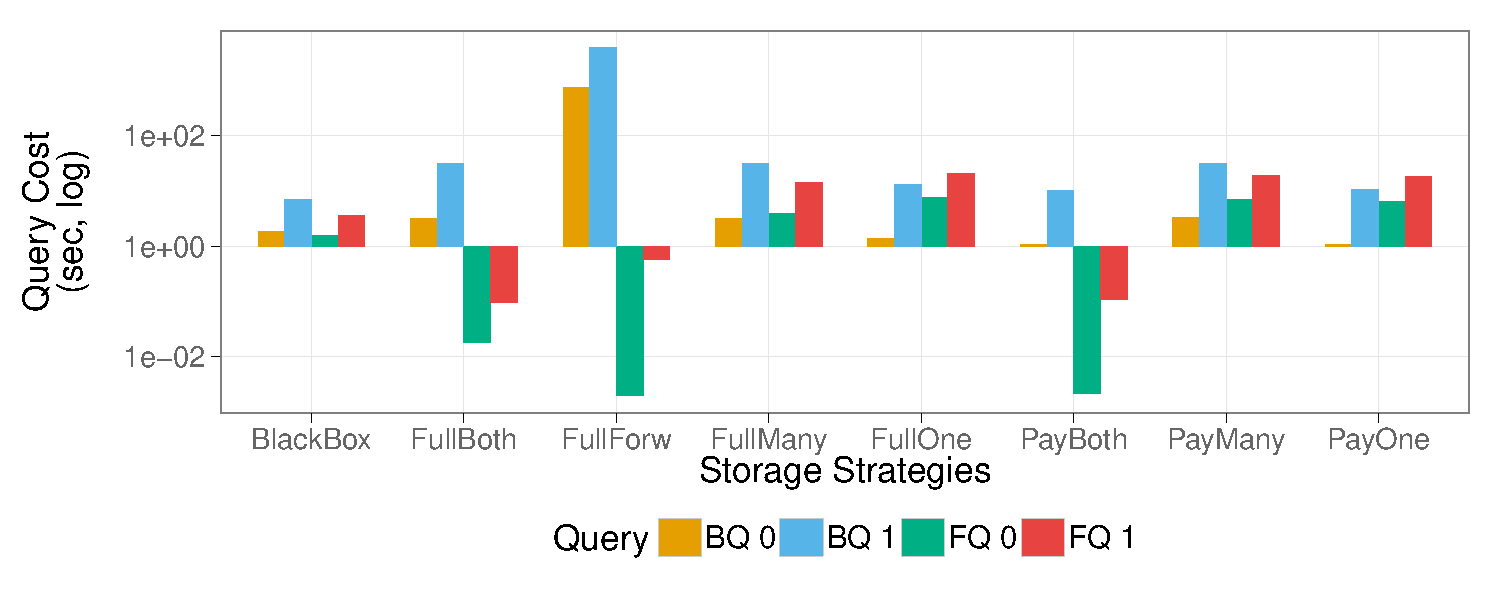
\includegraphics[width=3.5in,natwidth=10in,natheight=4in]{figures/genomics/cost_static.pdf}
}
\subfigure[Query costs (dynamic). Y-axes are log scale.]
{
    \label{f:gcosts100_dynamic}
     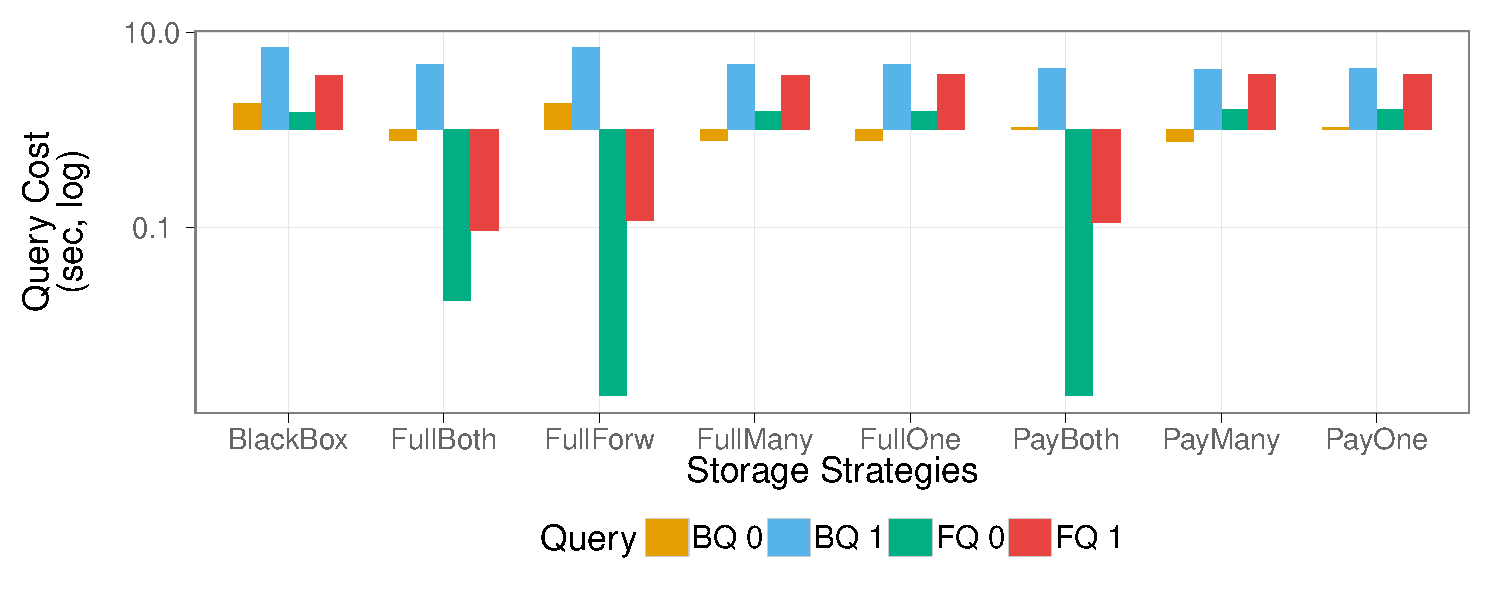
\includegraphics[width=3.5in,natwidth=10in,natheight=4in]{figures/genomics/cost_dynamic.pdf}
}
\advance\rightskip-.2in
\caption{Genomics benchmark.  Queries run
  with (dynamic) and without (static) the query-time optimizer
  described in Section \ref{s:cmopt}.}
\label{f:genomics1}
\end{figure}

In this experiment, we run the genomics workflow and execute a
lineage workload with an equal mix of forward and backward
lineage queries (Section \ref{s:ucgenomics}).  There are 10
built-in mapping operators, and the 4 UDFs are all payload operators.
In contrast to the astronomy workflow, these UDFs do not exhibit
significant locality, and perform data shuffling and extraction
operations that are not amenable to mapping functions.  In addition,
the operators perform simple calculations, and execute quickly, so
there is a less pronounced trade off between re-executing the workflow
and accessing region lineage.  In fact, there are cases where
storing lineage actually {\it degrades} the query performance.  We
were provided a 56$\times$100 matrix of 96 patients and 55 health and
genetic features.  Although the dataset is small, future datasets are
expected to come from a larger group of patients, so we constructed
larger datasets by replicating the patient data. The
query performance and overheads scaled linearly with the size of the
dataset and so we report results for the dataset scaled by 100$\times$.

We first show the high variability between different static strategies (Table
\ref{t:strats}) and how the query-time optimizer (Section~\ref{s:cmopt})
avoids sub-optimal query execution.  We then show how the \sys{} cost based
optimizer can identify the optimal strategy within varying user constraints.



\subsubsection{Query-Time Optimizer}
\label{s:genomicsfixed}

This experiment compares the strategies in Table~\ref{t:strats} with and
without the query-time optimization described in Section~\ref{s:cmopt}.  Each
operator uses mapping lineage if possible, and otherwise stores lineage
using the specified strategy.  The majority of the UDFs generate region pairs
that contain a single output cell.  As mentioned in previous experiments,
payload lineage stores very little binary data, and incurs less overhead
than the full lineage approaches (Figure~\ref{f:goverhead}).  Storing both
forward and backward-optimized lineage ($PayBoth$ and $FullBoth$) requires
significantly more overhead --  8 and 18.5$\times$ more space than the input
arrays, and 2.8 and 26$\times$ runtime slowdown.

Figure \ref{f:gcosts100_static} highlights how query performance can {\it
degrade} if the executor blindly joins queries with mismatched indexed lineage
(e.g., backward-optimized lineage with forward queries)\footnote{ All
comparisons are relative to $BlackBox$}.  For example, $FullForw$ degraded
backward query performance by 520$\times$.  Interestingly, the BQ1 ran slower
because the query path contains several operators with very large fanins.  This
generates so many intermediate results that performing index lookups on each
one is slower than re-running the operators.  Note however, that the forward
optimized strategies improved the performance of FQ0 and FQ2 because the fanout
is low.

Figure~\ref{f:gcosts100_dynamic} shows that the query-time optimizer executes
the queries as fast as, or faster than, $BlackBox$. In general, this
requires accurate statistics and cost estimation, the optimizer limits the
query performance degradation to 2$\times$ by dynamically switching to the
$BlackBox$ strategy.  Overall, the backward and forward queries improved by up
to 2 and 25$\times$, respectively.








\subsubsection{Lineage Strategy Optimizer}

\begin{figure}[tb]
\vspace{-.1in}
\advance\leftskip-.05in
\subfigure[Disk and runtime overhead]
{
    \label{f:goverhead_opt}
     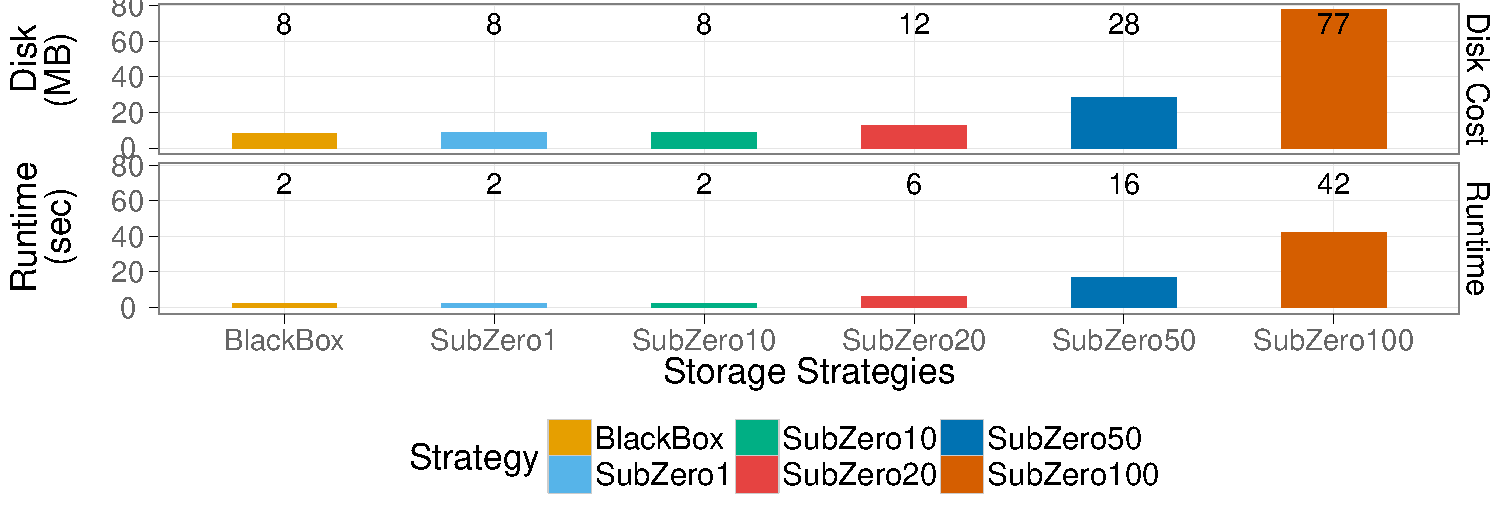
\includegraphics[width=3.5in,natwidth=10in,natheight=3.5in]{figures/genomics/overhead_opt.pdf}
}
\subfigure[Query costs.  Y-axes are log scale.]
{
    \label{f:gcosts100_opt}
     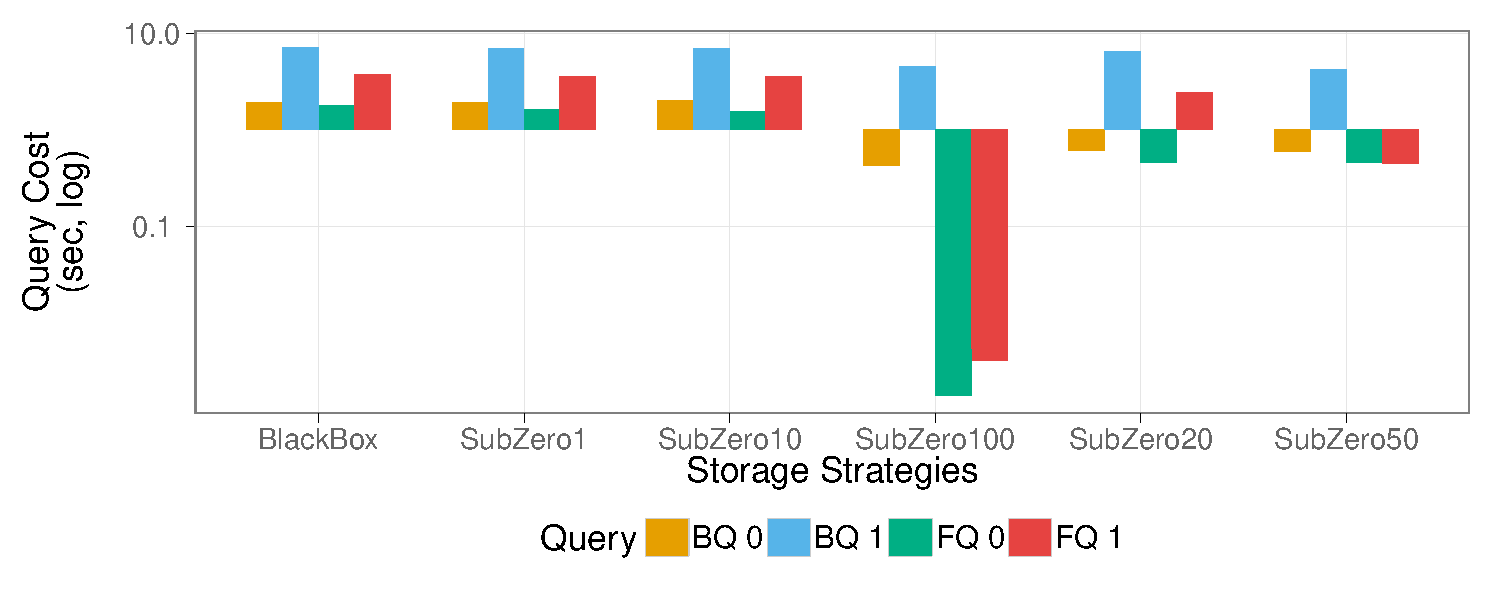
\includegraphics[width=3.5in,natwidth=10in,natheight=4in]{figures/genomics/cost_opt.pdf}
}
\advance\rightskip-.2in
\caption{Genomics benchmark.  SubZero{\it X} has storage constraint {\it X} MB }
\vspace{.1in}
\label{f:goptimizer}
\end{figure}



The previous section compared many strategies, each with different performance
characteristics depending on the operator and query.  We now evaluate the
\sys{} strategy optimizer on the genomics benchmark. Figure \ref{f:goptimizer}
illustrates that when the user increases storage constraints from 1 to 100MB
(with unbounded runtime constraint), the optimizer picks more storage intensive
strategies that are predicted to improve the benchmark queries.  \sys{} chooses
$BlackBox$ when the constraint is too small, and stores forward and
backward-optimized lineage that benefits all of the queries when the minimum
amount of storage is available (20MB).  Materializing further lineage has
diminishing storage-to-query benefits.  $SubZero100$ uses 50MB to
forward-optimize the UDFs using $(MANY, ONE)$, which reduces the forward query
costs to sub-second costs. This is because the UDFs have low fanout, so each
join in the query path is a small number of hash lookups.  Due to space
constraints, we simply mention that specifying and varying the runtime overhead
constraints achieves similar results.




\subsection{Microbenchmark}


The previous experiments compared several end-to-end strategies, however it can
be difficult to distinguish  the sources of the benefits.  This
subsections summarizes the key differences between the prevailing strategies in
terms of overhead and query performance.  The comparisons use an operator that
generates synthetic lineage data with tunable parameters.  Due to space
constraints we show results from varying the fanin, fanout and payload size
(for payload lineage).


%for the lineage
%fanin and fanout ($fanin$ \& $fanout$), the payload size for payload lineage,
%and the number of output cells containing lineage that are generated
%($noutput$).  Due to space constraints we report results where $noutput=10\%$
%of the output array.  The results scale close to linearly with $noutput$.

Each experiment processes and outputs a 1000x1000 array, and generates lineage
for 10\% of the output cells.  The results scaled close to linearly as the
number of output cells with lineage varies.   A region pair is
randomly generated by  selecting a cluster of output cells with a radius
defined by $fanout$, and selecting $fanin$  cells in the same area from the
input array.   We generate region pairs until the total number of output cells
is equal to 10\% of the output array.  The payload strategy uses a payload size
of {\it fanin}$\times${\it 4 bytes} (the payload is expected to be very small).
We compare several backward optimized strategies ($\leftarrow FullMany$,
$\leftarrow FullOne$, $\leftarrow PayMany$, $\leftarrow PayOne$), one forward
lineage strategy ($\rightarrow FullOne$), and black-box ($BlackBox$).   We
first discuss the overhead to store and index the lineage, then comment on
the query costs.


Figure \ref{f:micro_overhead} compares the runtime and disk overhead of the
different strategies.  For referenc, the size of the input array is 3.8MB.  The
best full lineage strategy differs based on the operator fanout. $FullOne$ is
superior when $fanout \le 5$ because it doesn't need to create and store the
spatial index.  The crossover point to $FullMany$ occurs when the cost of
duplicating hash entries for each output cell in a region pair exceeds that of
the spatial index.  The overhead of both approaches increases with fanin.  In
contrast, payload lineage has a much lower overhead than the full lineage
approaches and is independent of the fanin because the payload is typically
small and does not need to be encoded.  When the fanout increases to 50 or 100,
$PayMany$ and $FullMany$ require less than 3MB and 1 second of overhead.
 The forward optimized $FullOne$ is comparable to
the other approaches when the fanin is low.   However, when the fanin increases
it can require up to $fanin\times$ more hash entries because it creates an
entry for every distinct input cell in the lineage.  It converges to the
backward optimized $FullOne$ when the fanout and fanin are high. Finally,
$BlackBox$ has nearly no overhead.

Figure \ref{f:micro_query} shows that the query performance for queries that
access the backward/forward lineage of 1000 output/input cells.  The
performance scales mostly linearly with the query size.  There is a clear
difference between $FullMany$ or $PayMany$, and $FullOne$ or $PayOne$, due to
the additional cost of accessing the spatial index (Figure
\ref{f:micro_query}).  Payload lineage performs similar to, but not
significantly faster than full provenance, although the query performance
remains constant as the fanin increases.    In comparison (not shown),
$BlackBox$ takes between 2 to 20 seconds to execute a query where {\it fanin=1}
and around 0.7 seconds when {\it fanin=100}.  Using a mis-matched index (e.g,
using forward-optimized lineage for backward queries) takes up to two orders of
magnitude longer than $BlackBox$ to execute the same queries.  The forward
queries using $\rightarrow FullOne$ execute similarly to $\leftarrow FullOne$
in Figure~\ref{f:micro_query} so we do not include the plots.
%\srm{Figure  \ref{f:micro_query}(b) is pretty boring, since you aren't
%comparing anything!}

%\begin{figure}[ht]
%\advance\leftskip-.3in
%\subfigure[Disk Overhead]
%{
%    \label{f:micro_disk}
%    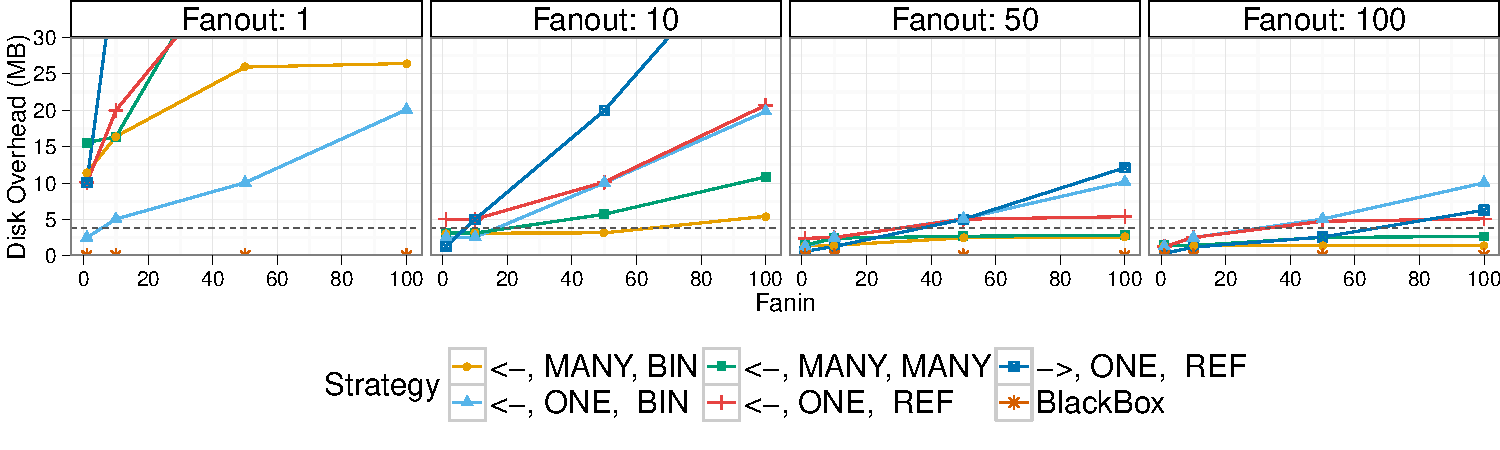
\includegraphics[width=3.7in]{figures/microbench/disk}
%}\\
%\subfigure[Runtime Overhead]
%{
%    \label{f:micro_runtime}
%    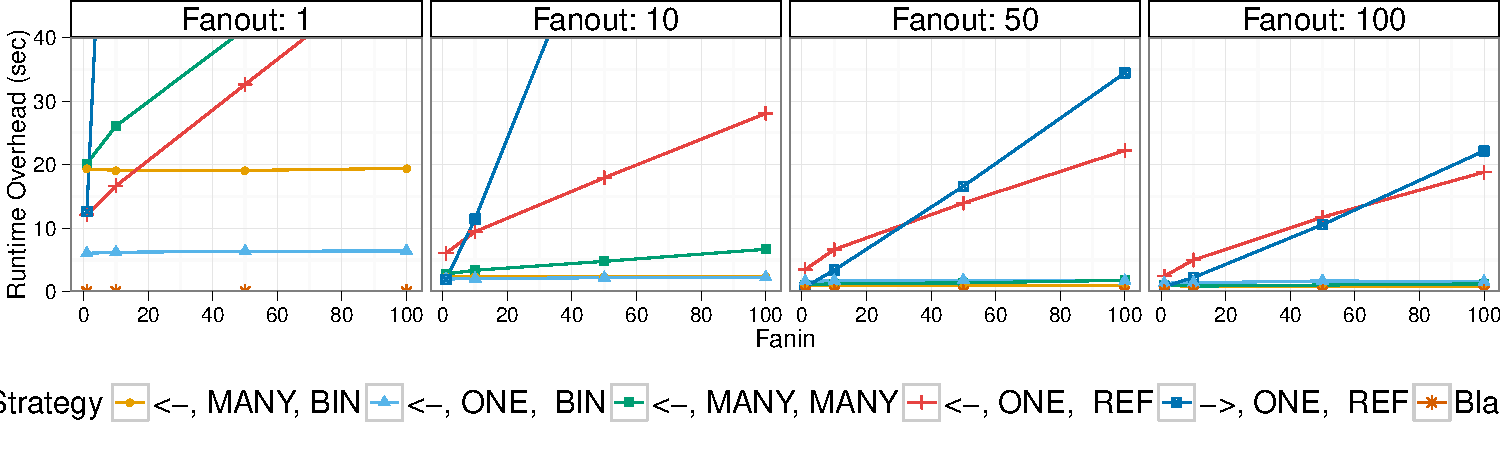
\includegraphics[width=3.7in]{figures/microbench/runtime}
%}
%%\advance\rightskip-.2in
%\vspace{-.2in}
%\caption{Disk and runtime overhead}
%\label{f:micro_overhead}
%\end{figure}


\begin{figure}[ht]
%\advance\leftskip-.2in
    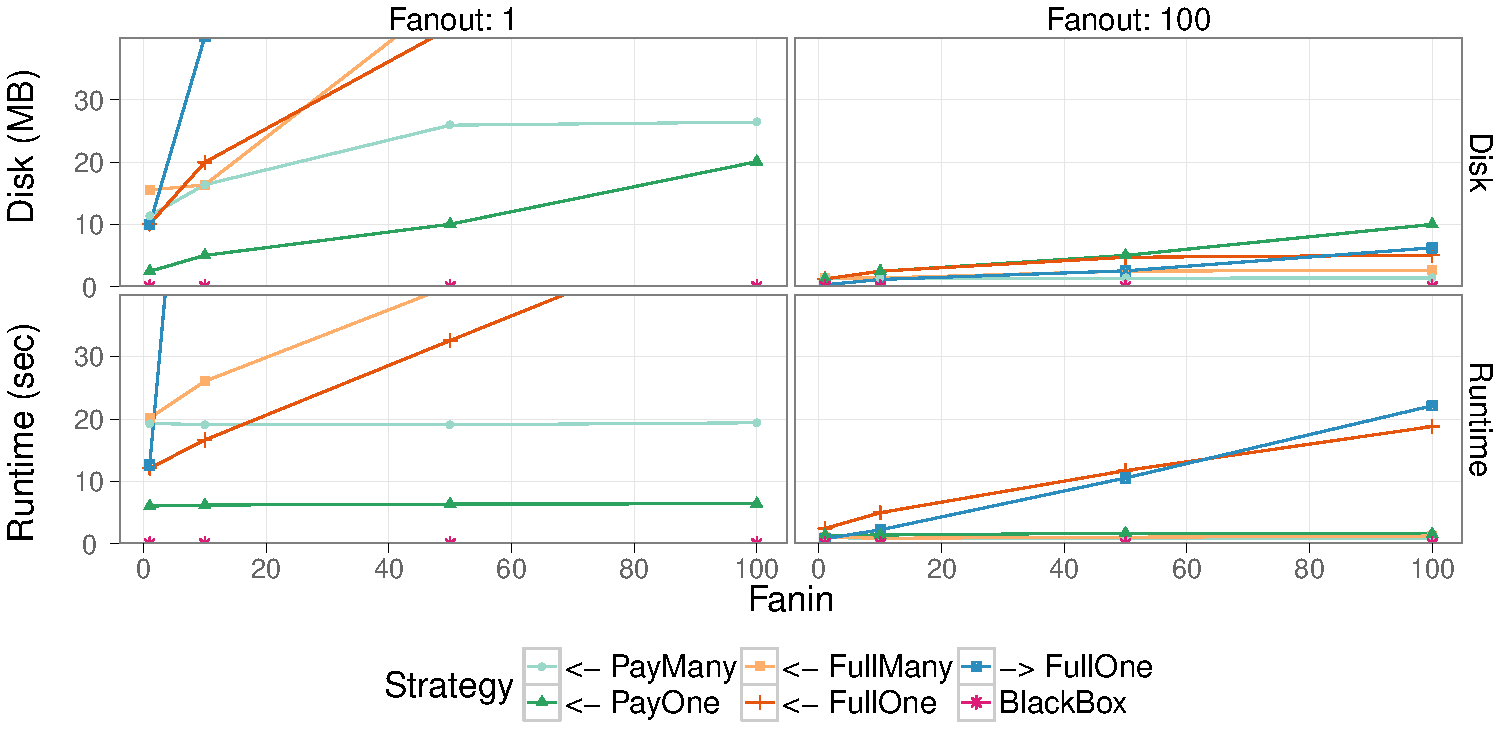
\includegraphics[width=3.7in,natwidth=10in,natheight=5in]{figures/microbench/overhead.pdf}
%\advance\rightskip-.2in
\vspace{-.2in}
\caption{Disk and runtime overhead}
\label{f:micro_overhead}
\end{figure}

\begin{figure}[htb]
%\advance\leftskip-.3in
    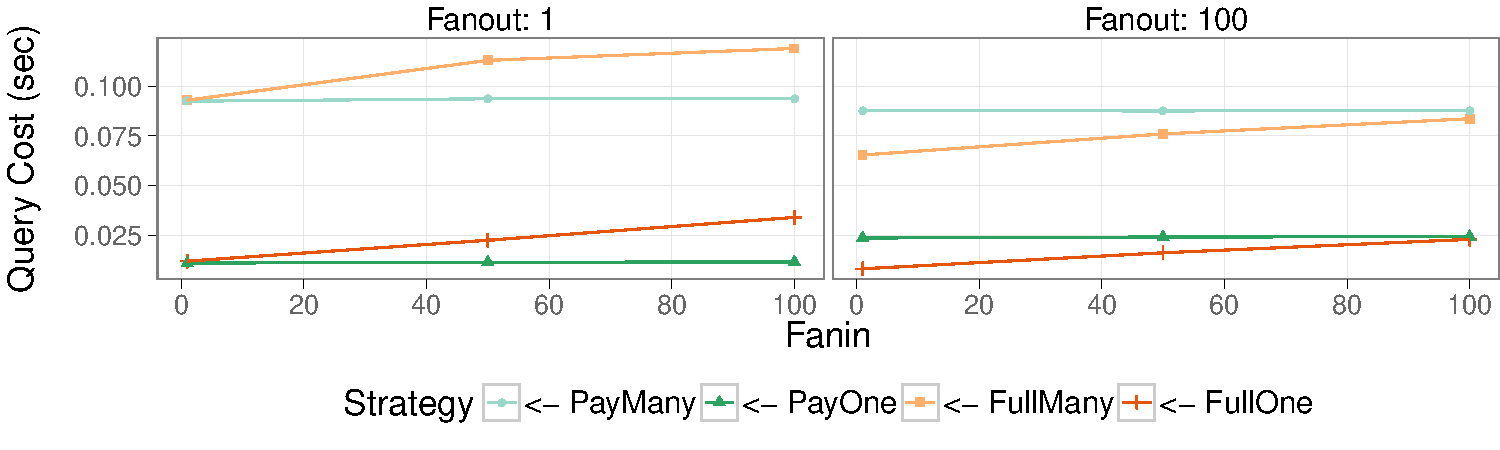
\includegraphics[width=3.6in,natwidth=10in,natheight=3in]{figures/microbench/query_back.pdf}
%\advance\rightskip-.2in
%\vspace{-.2in}
\caption{Backward Lineage Queries, only backward-optimized strategies}
\label{f:micro_query}
\end{figure}




%\begin{figure}[htb]
%%\advance\leftskip-.3in
%\subfigure[Backward Queries, only backward-optimized strategies]
%{
%    \label{f:micro_bq}
%    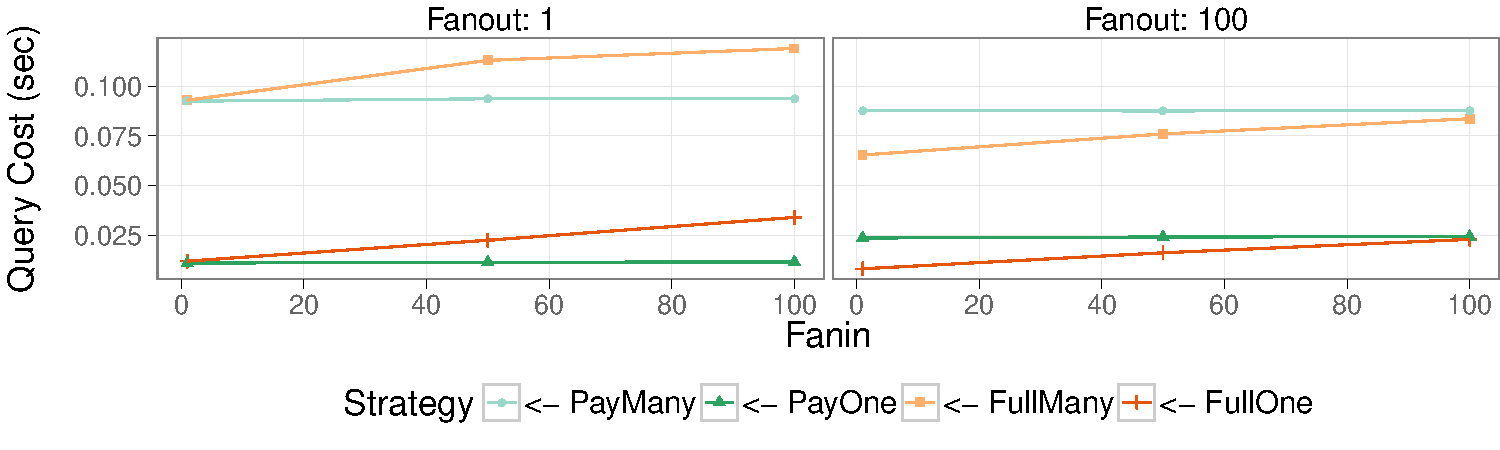
\includegraphics[width=3.6in]{figures/microbench/query_back}
%}\\
%\subfigure[Forward Queries, only forward-optimized strategies]
%{
%    \label{f:micro_fq}
%    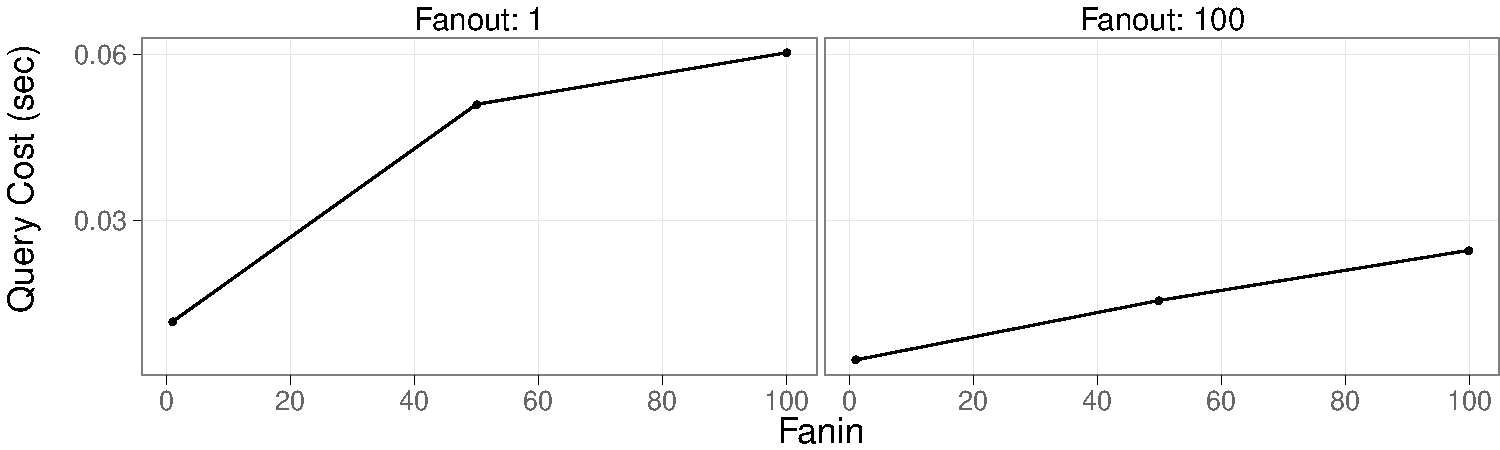
\includegraphics[width=3.6in]{figures/microbench/query_forw}
%}
%%\advance\rightskip-.2in
%%\vspace{-.2in}
%\caption{Backward and Forward lineage query costs.}
%\label{f:micro_query}
%\end{figure}



%The storage strategy is tied to the lineage queries and user preferences
%between workflow execution overhead and lineage query performance.  Poorly
%designed systems can easily incur three orders of magnitude of runtime
%overhead, 4$\times$ the disk overhead, and two orders of magnitude query slow
%down.




\subsection{Discussion}

The experiments show that the best strategy is tied to the
operator's lineage properties, and that there are orders of magnitude
differences between different lineage strategies.   Science-oriented lineage
systems should seek to identify and exploit operator fanin, fanout, and
redundancy properties.

Many scientific applications -- particularly sensor-based or image processing
applications like environmental monitoring or astronomy -- exhibit substantial
locality (e.g., average temperature readings within an area) that can be used
to define payload, mapping or composite operators.  As the experiments show,
\sys{} can  record their lineage with less overhead than from operators that
only support full lineage. When locality is not present, as in the genomics
benchmark,  the optimizer may still be able to find opportunities to record
lineage if the constraints are relaxed.  A very promising alternative is to
simplify the process of writing payload and mapping functions by supporting
variable granularities of lineage.  This lets developers define coarser
relationships between input and outputs (e.g., specify lineage as a bounding
box that may contain inputs that didn't contribute to the output). This also
allows the lineage system perform lossy compression.

%The experiments showed that the slowdown caused by  storing lineage
%can dwarf the cost of executing the application (e.g., the genomics benchmark),
%which is unacceptable in scenarios such as real-time applications.  In these
%cases, the optimizer will choose black-box lineage.  However, as evidenced in
%the genomics benchmark and the microbenchmarks, \sys{} can still improve query
%peformance by efficiently store lineage for high fanout operators or operators
%that support payload lineage.

%Although our region provenance encodings are applicable to a large class of
%scientific operators, if may be difficult to define  mapping functions or  the
%correct $lwrite$ calls for complex UDFs.  In these cases, the developer may opt
%to adopt a coarser definition of lineage by specifying coarse regions of input
%cells. While out of the scope of this paper, supporting and optimizing varying
%granularities of lineage is a promising future direction.


%Finally, there may be times where the lineage is very expensive to store but is
%not  {\it useful} (e.g., kmeans just references everything), and sometimes the
%lineage is very large, which motivates the DBWipes stuff we are doing. Maybe we
%should just reference what we're doing as ``future work?''}


%
%The microbenchmarks showed that the runtime overhead increases as more
%lineage is stored. For example, the runtime overhead was up to 50$\times$ in
%the genomics benchmark. This may be unacceptable for applications with
%real-time requirements (forcing our optimizer to choose to just use black box
%lineage).  However, even strict constraints can provide benefits -- the
%$PayOne$ strategy in Figure~\ref{f:genomics1}(c) reduced backwards query costs
%by about 50\% while imposing a very small runtime penalty.  Other applications,
%such as the genomic visualization that interactively executes lineage
%queries, may be willing to incur offline overhead in order to minimize query
%runtimes.

%We also note that many scientific applications -- particularly sensor-based or
%image processing applications like environmental monitoring or astronomy --
%exhibit substantial locality (e.g., average temperature readings within an
%area) that can be used to define payload, mapping or composite operators.


%\red{Highlight how powerful composite lineage is.  Talk about
%    programmability -- many readers will worry that some operators are simply
%    very difficult write $lwrite$ functions for.  I actually think that many
%    UDFs may be very complicated, but the input to output relationships should
%    ultimately be pretty obvious (perhaps at a coarser grain).  Often

